\section{Lime}

\begin{frame}
	\begin{block}{Artigo 01}
	\begin{enumerate}
		\item ``Why Should I Trust You?'' Explaining the Predictions of Any Classifier
	\end{enumerate}
	\end{block}
\end{frame}


\begin{frame}
	\begin{block}{Lime - overview}
	\begin{enumerate}
		\item É agnóstico (não assume nada sobre o modelo, dessa forma, funciona para qualquer modelo)
		\item Realiza uma interpretação Local do score gerado pelo modelo.
		\item Um ponto falho é que a interpretação foi avaliada usando modelos pequenos (até 10 features) interpretáveis (explicar por que é falho) 
		\item Um ponto fraco da técnica é que a função de distância depende do tipo de dado de input (texto, imagem, numérico...)
	\end{enumerate}
	\end{block}
\end{frame}


\begin{frame}
	\begin{block}{Lime - funcionamento}
		\begin{enumerate}
			\item Escolhe uma instância que deseja interpretar
			\item Seleciona outras instâncias próximas a ela (usando uma métrica de distância D)
			\item Usando a amostra executa uma logística para aprender, localmente, quais as variáveis mais importantes
		\end{enumerate}
	\end{block}
\end{frame}


\begin{frame}
	\begin{block}{Lime - fronteira de decisão}
		\begin{figure}[!htb]
			\centering	  				
			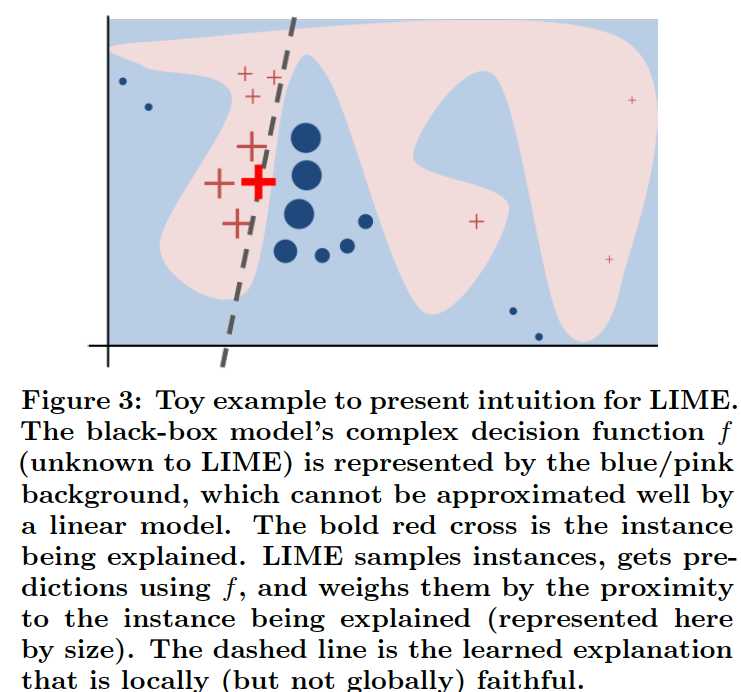
\includegraphics[height=4cm, width = 10cm]{./pic/LIMEfronteira.png}
			\caption{LIME fronteira de decisão}
			\label{fig_ds_process}
		\end{figure}	
	\end{block}
\end{frame}





